\begin{figure}
    \centering
    \begin{subfigure}[b]{\linewidth}
    \centering
    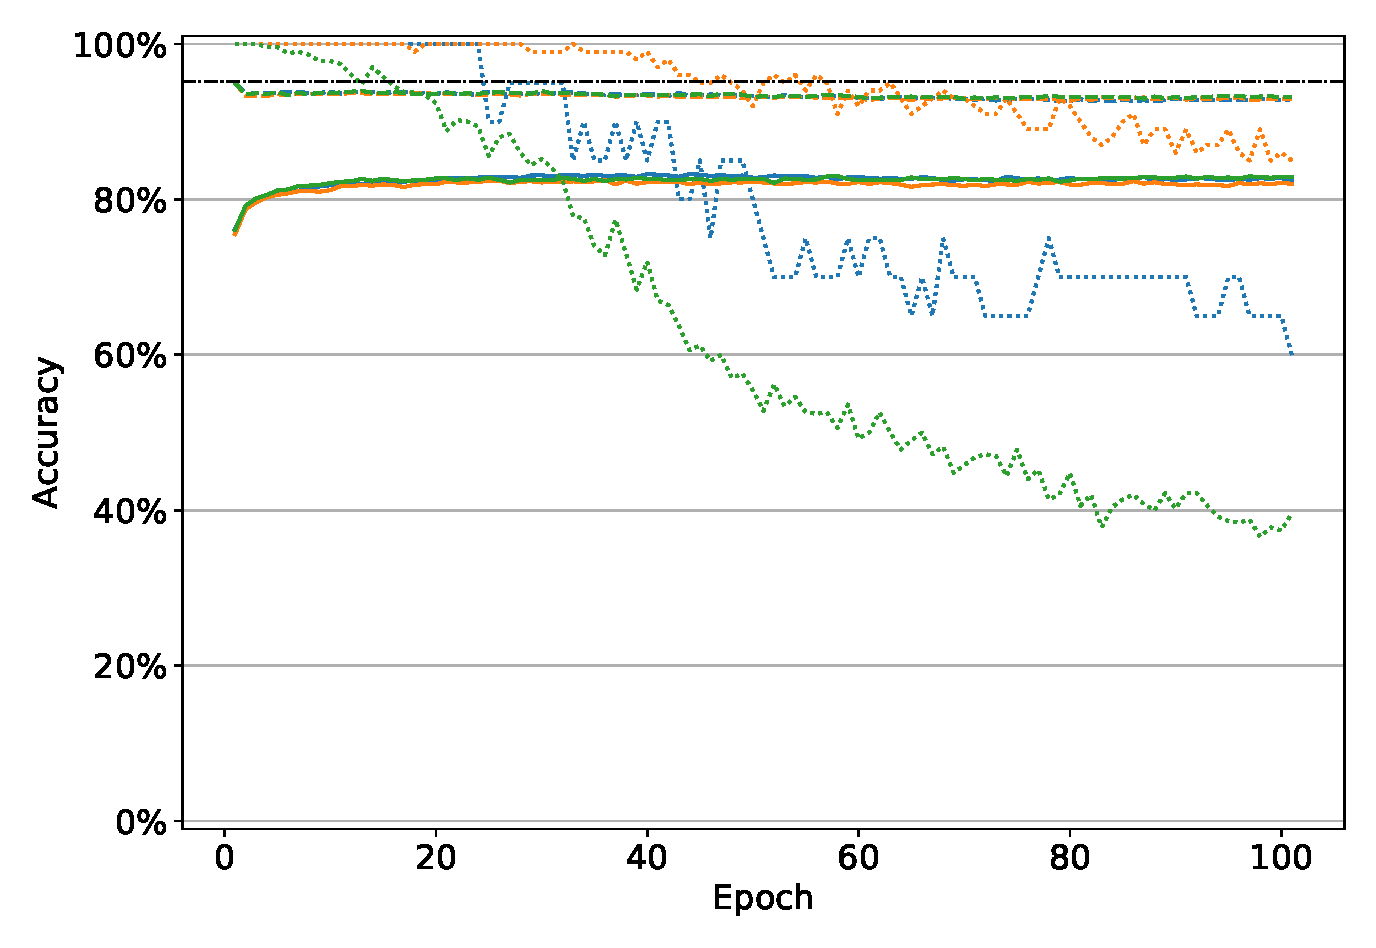
\includegraphics[width=0.7 \linewidth]{images/finetuning/finetuning_protecting_content_trgsetsizes_thesis_resnet18.eps}
    \end{subfigure}
    \begin{subfigure}[b]{\linewidth}
    \centering
    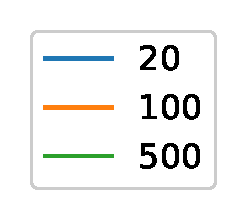
\includegraphics[height=1cm]{images/finetuning/legend_finetuning_protecting_content_trgsetsizes_colors.eps}
    \quad
    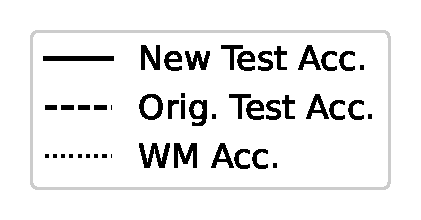
\includegraphics[height=1cm]{images/finetuning/legend_finetuning_protecting_content_trgsetsizes_linetypes.eps}
    \end{subfigure}
    \caption{Behaviour of ResNet-18 watermarked with \textit{ProtectingIP-pattern} during a fine-tuning attack with a small learning rate $\alpha=10^{-4}$. The colors indicate the trigger set size, with which the model was watermarked. The black dash-dotted line corresponds to the benchmark test accuracy of the non-watermarked model.}
    \label{fig:finetuning-content-trgsetsizes}
\end{figure}